\chapter{The physical Track}

Being able to drive along a simulation of the track is only a partial success. In order to prove successful, the trained algorithm is required to complete multiple runs on a real track using our DeepRacer vehicle. We decided on rebuilding the track used 2018 during the AWS re:Invent. The circular track starts with a 180° left turn, followed by a right-starting s-curve and continues on with two left turns back to the beginning. With a total width of 7.93 m and length of 5.18 m it impractical to paint it on a single, solid piece.

\begin{figure}
    \centering
    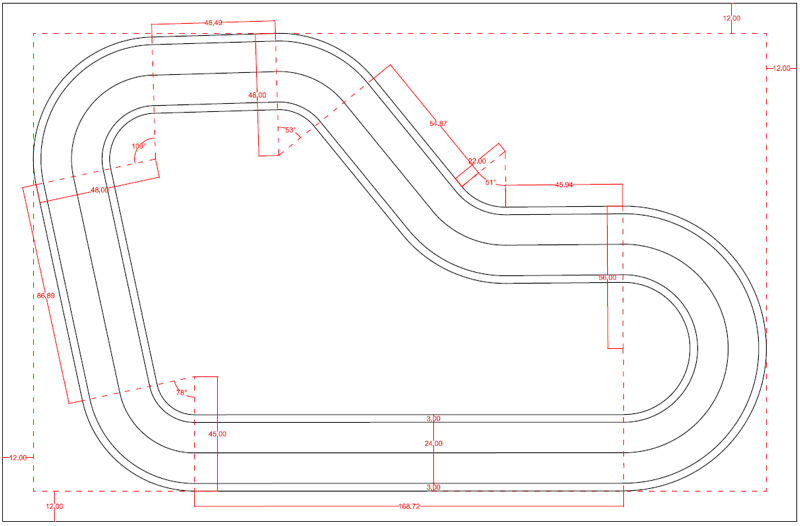
\includegraphics[width=.85\textwidth]{deepracer-track-2018-guideline.png}
    \caption{AWS re:Invent 2018 track}
    \label{fig:track}
\end{figure}

Before we considered building the track, we drew it on the floor in our robotics laboratory using duct tape. This was possible due to the floor being solid black, just like the road on the track. This variant has several drawbacks compared to a properly built track. Built like this the track is stationary and can not be removed without destroying parts of it. During removal it might even happen that the adhesive will leave stains on the floor, which then again need to be removed. The alternative, interlocking foam pieces, are transportable and more durable, as they can be easily removed and rebuild as needed. Their major drawback is the costs. While using duct tape as markings on the floor is cheaper and faster, using foam puzzles will be more efficient in the long run.

\section{The Material}
Choosing the right material for the track proved to be straightforward. It came down to either interlocking wooden composite plates or interlocking foam pieces. Foam pieces provide many advantages compared to other materials. They are lightweight and easy to transport. Durability and thickness are not as important, as the track is not meant to be stepped on and our car does not weight a lot. Far more important is the ability of the pieces to stick together. The tiles must not under any circumstances break away from each other, this could cause serious damage to the track and vehicle. Interlocking foam tiles are the cheapest material still meeting all criteria, with the only drawback being the cost.

\subsection{Track and Field Colour}

